%++++++++++++++++++++++++++++++++++++++++
% Don't modify this section unless you know what you're doing!
\documentclass[letterpaper,12pt]{article}
\usepackage{tabularx} % extra features for tabular environment
\usepackage{amsmath}  % improve math presentation
\usepackage{graphicx} % takes care of graphic including machinery
\usepackage{subcaption}
\usepackage{mathtools}
\usepackage[margin=1in,letterpaper]{geometry} % decreases margins
\usepackage{cite} % takes care of citations
\usepackage[final]{hyperref} % adds hyper links inside the generated pdf file
\usepackage{titlesec} % enable 1.1.1.1
\setcounter{secnumdepth}{4}
\hypersetup{
	colorlinks=true,       % false: boxed links; true: colored links
	linkcolor=blue,        % color of internal links
	citecolor=blue,        % color of links to bibliography
	filecolor=magenta,     % color of file links
	urlcolor=blue         
}
\DeclarePairedDelimiterX{\norm}[1]{\lVert}{\rVert}{#1}
%++++++++++++++++++++++++++++++++++++++++


\begin{document}

\title{Team 07 - Update 2 \\
	   \large CS6220 - Data Mining Techniques - Fall 2017 \\
	   \large Northeastern University}
\author{Nakul Camasamudram, Rosy Parmar, Rahul Verma, Guiheng Zhou}
\date{\today}
\maketitle


\section{Introduction}
We are building a recommender system that provides personalized recommendations based on prior implicit feedback using ”The Instacart Online Grocery Shopping Dataset 2017”. Instacart is an American company that operates as a same-day grocery delivery service. This anonymized dataset contains a sample of over 3 million grocery orders from more than 200,000 Instacart users.

\subsection{Data Analysis}

Orders from Instacart are available in four .csv files: "orders.csv", "order\_products\_\_train.csv", "order\_products\_\_prior.csv" and "sample\_submission.csv". The key to understanding the dataset and the train/test split is the orders table ("orders.csv").

Take for example User 1[Fig 1] , who happens to be a train user. User 1 has 10 prior orders, and 1 train order whose details are provided in "order\_products\_\_prior.csv" and in "order\_products\_\_train.csv" respectively.

\begin{figure}[!bp]
  \begin{subfigure}[b]{0.4\textwidth}
    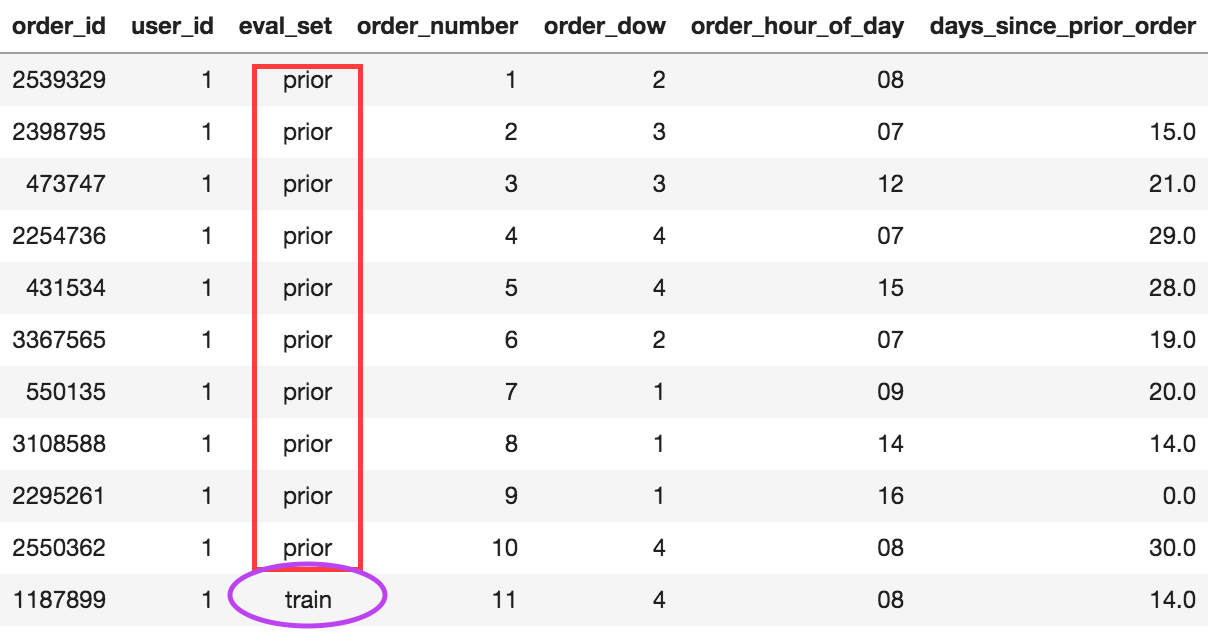
\includegraphics[width=\textwidth]{train_user.png}
    \caption{User 1}
    \label{fig:f1}
  \end{subfigure}
  \hfill
  \begin{subfigure}[b]{0.4\textwidth}
    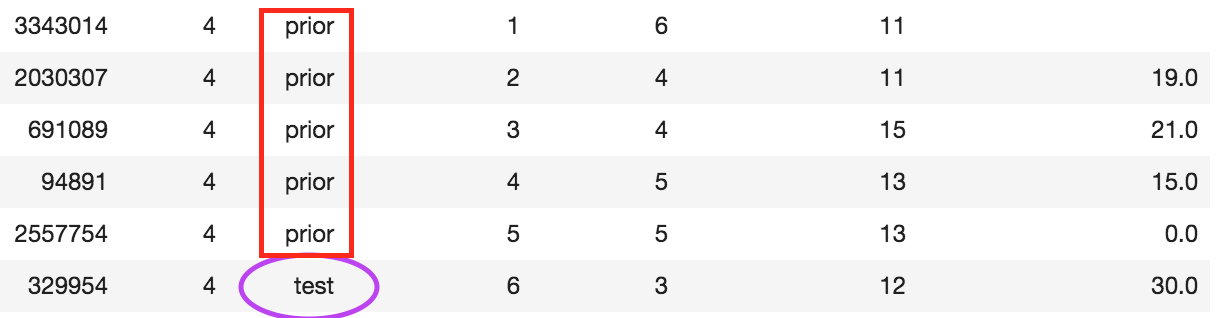
\includegraphics[width=\textwidth]{test_user.png}
    \caption{User 4}
    \label{fig:f2}
  \end{subfigure}
  \caption{Train/Test Split}
\end{figure}

Similarly, User 4 is a test user. He has 5 prior orders, and his 6th is a test order. Their details are available in "order\_products\_\_prior.csv" and "sample\_submission.csv" respectively.

Figure 2 is a glimpse at "order\_products\_\_prior.csv" when merged with three other .csv files that represent products, aisles and departments. The format of "sample\_submission.csv" and "order\_products\_\_train.csv" is exactly the same.

\begin{figure*}
	\centering
	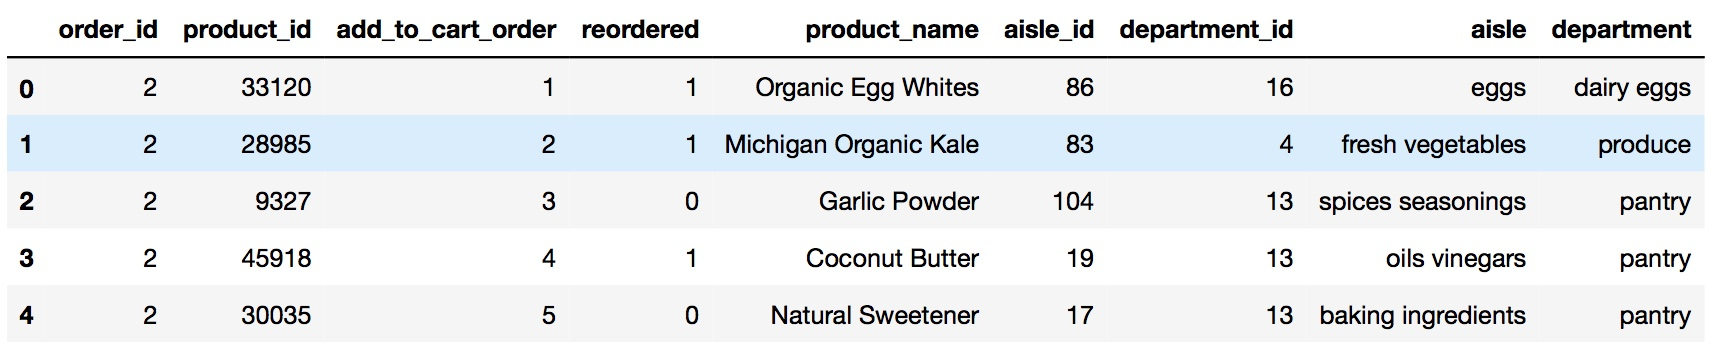
\includegraphics[scale=0.2]{prior_df_merged} \\
	\caption{Merged Prior Orders}
\end{figure*}	


The below figures depicts the product frequency distribution across orders as well as the most popular products. The "long tail" phenomenon is clearly visible in the former.
\begin{center}
	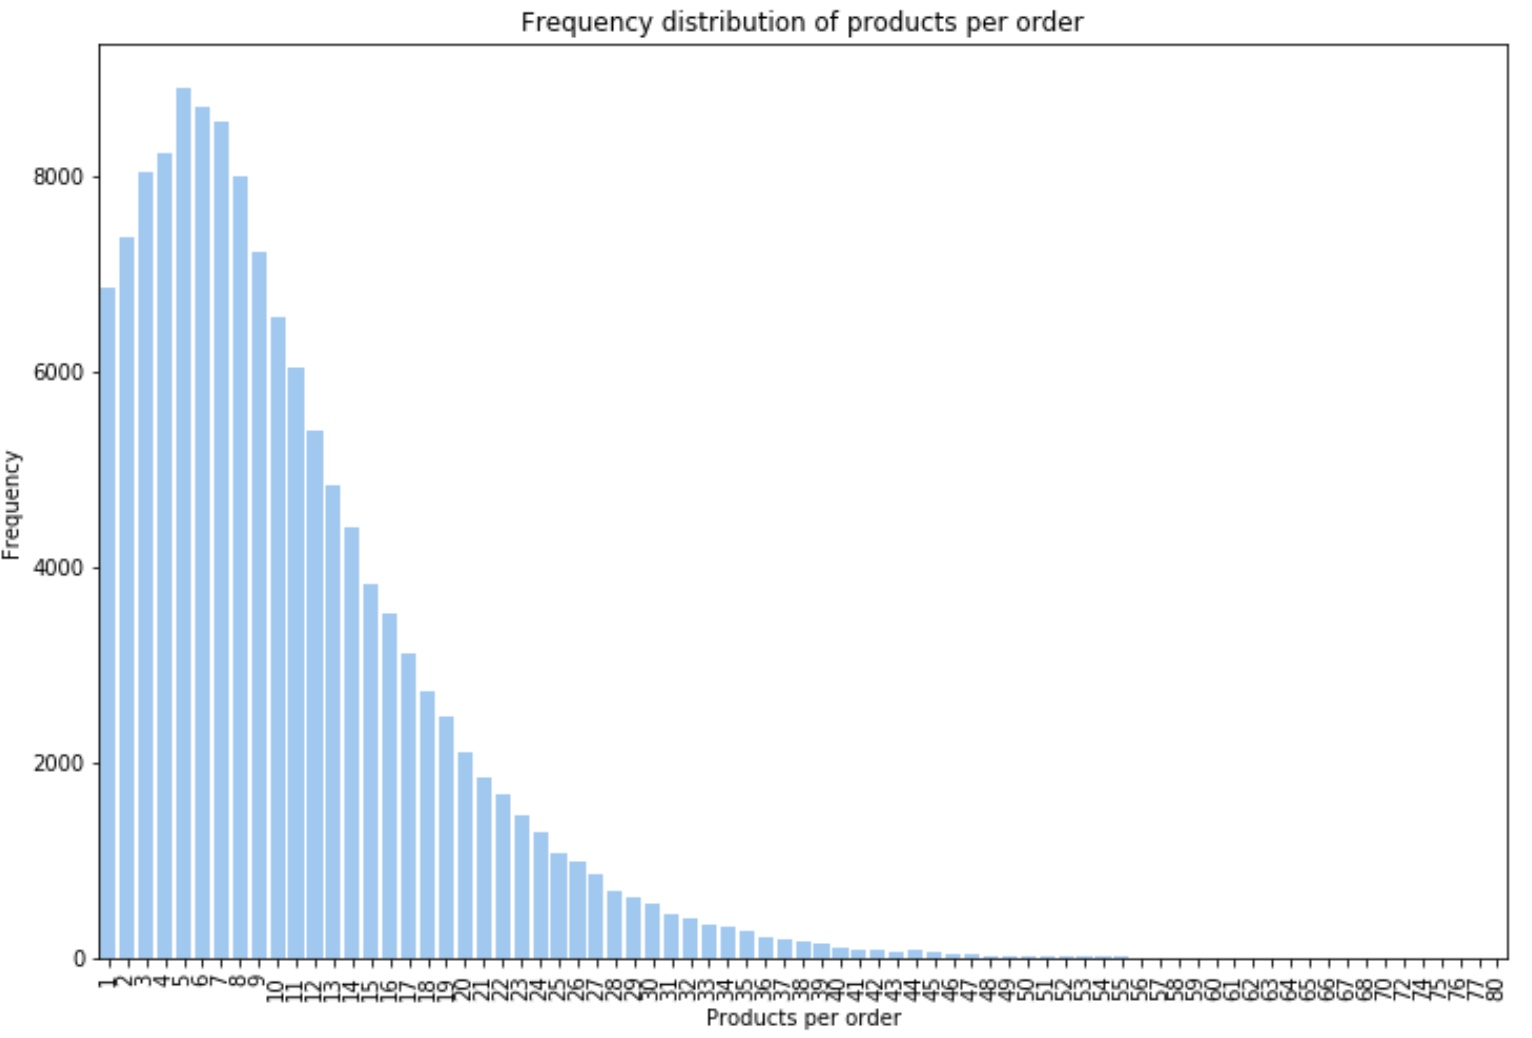
\includegraphics[scale=0.2]{train_products_order}
\end{center} 

\begin{center}
	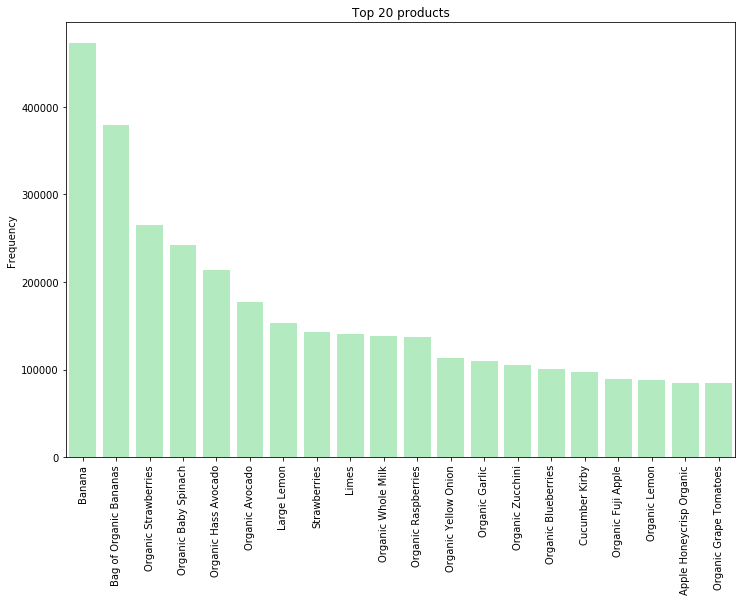
\includegraphics[scale=0.4]{top_20_products.png}
\end{center}


\subsection{Challenges}
We are using algorithms specifically suited for processing implicit feedback. It is important to highlight unique characteristics of implicit feedback, which prevent the application of algorithms that were designed for explicit feedback data.

\begin{enumerate}
	\item The dataset has information about users prior purchases from which we can infer what they like. However, there is no concrete metric to deduce what a user dislikes.
	\item Just because a user purchased a product, does not necessarily mean he/she likes the product. The purchase could've been made as a gift or perhaps after receiving the product, the user might've been disappointed with it. Also, the frequency of product purchases doesn't necessarily indicate a user's preference, it's more of an indicator for a user's confidence in the product. Hence, a user's true preferences can only be guessed.
	\item Systems dealing with explicit feedback are generally evaluated using metrics such as mean average error. With implicit systems, the recommender's output is compared with a user's current purchase on the test set using set based measures.
\end{enumerate}

\section{Approaches}

\subsection{Reviewed Approaches}

\subsection{Neighborhood-based Methods}
\subsubsection{Term Frequency-Inverse Document Frequency (tf-idf)}
\paragraph{Basic Idea}\mbox{}\\
In this method, we made an analogy between the documents and user purchase histories, and between the terms and the products users purchased. Term frequency is represented by the number of occurrences of an 

\subsubsection{Word2Vec Similar Product/Similar User Based Model}
With the help of Word2Vec we have done these 2 tasks:
\\\\ 1. Finding Similar Users to a User.
		a. We do this by first making a list of procuts purchased in an order as a numpy se
\\\\ 2. Finding Products similar to a product.

\subsection{Latest Factor Methods}

\subsubsection{Implicit Alternating Least Squares\cite{implicitals}}

The key idea of the implicit ALS is to transform a user item matrix of product purchase frequencies to a confidence matrix $C_{ui}$ for users $u$ and items $i$.

\begin{equation*}
	C_{ui} = 1 + \alpha R_{ui}
\end{equation*}

$\alpha$ represents a linear scaling of the rating preferences (in our case number of purchases) and $R_{ui}$ is the original matrix of purchases. The paper suggests $\alpha = 40$ to be a good starting point.

Now, similar to other matrix factorization methods, the goal is to find user-factor vectors $x_u\in{\rm I\!R}^{f}$ and item-factor vectors $y_i\in{\rm I\!R}^{f}$ for each user and item. These factors are computed by minimizing the cost function:

\begin{equation*}
	\min_{x, y} \sum_{u, i}{c_{ui}(p_{ui} - x_{u}^{T}y_{i})^2} + \lambda(\sum_{u}\norm{x_{u}}^2 + \sum_{i}\norm{y_{i}}^2)
\end{equation*}

This then leads to an alternating-least-square optimization process, where the algorithm alternates between re-computing user-factors and item-factors with each step guaranteed to lower the value of the cost.

In our case, we are using the library "implicit"\footnote{Fast Python Collaborative Filtering: https://github.com/benfred/implicit} to perform ALS optimization.

\section{Evaluation}

Recommendations for each user are ordered list of products, from the most preferred to the least preferred. The dataset has no feedback about product that are disliked and hence, precisiion based metrics are not appropriate. Instead, recall-oriented measures are applicable since a prior purchase of a product is an indication of liking it.

After training the respective models, we are generating recommendations for each user in the test dataset. We will then compute the mean recall over all the users in test dataset by comparing the actual current purchase of the user and the products recommended

\begin{equation*}
	\text{Mean Recall} = \sum_{\text{test users}} \frac{|\{\text{recommended}\}| \cap |\{\text{actual}\}|}{|\{\text{actual}\}|}
\end{equation*}


Furthermore, we will be evaluating all the models by comparing them to a baseline model that suggests the most popular items to every user.

\section{Next Steps}





%++++++++++++++++++++++++++++++++++++++++
% References section will be created automatically 
% with inclusion of "thebibliography" environment
% as it shown below. See text starting with line
% \begin{thebibliography}{99}
% Note: with this approach it is YOUR responsibility to put them in order
% of appearance.

\begin{thebibliography}{99}

\bibitem{implicitals}
Y.F. Hu, Y. Koren, and C. Volinsky, “Collaborative Filtering for Implicit Feedback Datasets,” Proc. IEEE Int’l Conf. Data Mining (ICDM 08), IEEE CS Press, 2008, pp. 263-272.


\bibitem{melissinos}
A.~C. Melissinos and J. Napolitano, \textit{Experiments in Modern Physics},
(Academic Press, New York, 2003).

\bibitem{Cyr}
N.\ Cyr, M.\ T$\hat{e}$tu, and M.\ Breton,
% "All-optical microwave frequency standard: a proposal,"
IEEE Trans.\ Instrum.\ Meas.\ \textbf{42}, 640 (1993).

\bibitem{Wiki} \emph{Expected value},  available at
\texttt{http://en.wikipedia.org/wiki/Expected\_value}.

\end{thebibliography}


\end{document}

